% Created 2017-01-11 mié 12:38
% Intended LaTeX compiler: pdflatex
\documentclass[xcolor={usenames,svgnames,dvipsnames}]{beamer}
\usepackage[utf8]{inputenc}
\usepackage[T1]{fontenc}
\usepackage{graphicx}
\usepackage{grffile}
\usepackage{longtable}
\usepackage{wrapfig}
\usepackage{rotating}
\usepackage[normalem]{ulem}
\usepackage{amsmath}
\usepackage{textcomp}
\usepackage{amssymb}
\usepackage{capt-of}
\usepackage{hyperref}
\usepackage{color}
\usepackage{listings}
\usepackage{mathpazo}
\usepackage{gensymb}
\usepackage{amsmath}
\bibliographystyle{plain}
\AtBeginSubsection[]{\begin{frame}[plain]\tableofcontents[currentsubsection,sectionstyle=show/shaded,subsectionstyle=show/shaded/hide]\end{frame}}
\AtBeginSection[]{\begin{frame}[plain]\tableofcontents[currentsection,hideallsubsections]\end{frame}}
\usepackage[emulate=units]{siunitx}
\sisetup{fraction=nice, decimalsymbol=comma, retain-unity-mantissa = false}
\newunit{\wattpeak}{Wp}
\newunit{\watthour}{Wh}
\newunit{\amperehour}{Ah}
\hypersetup{colorlinks=true, linkcolor=Blue, urlcolor=Blue}
\renewcommand{\thefootnote}{\fnsymbol{footnote}}
\setbeamercolor{alerted text}{fg=blue!50!black} \setbeamerfont{alerted text}{series=\bfseries}
\usetheme[hideothersubsections]{Goettingen}
\usecolortheme{rose}
\usefonttheme{serif}
\author{Oscar Perpiñán Lamigueiro \\ \url{http://oscarperpinan.github.io}}
\date{}
\title{Módulo y Generador}
\subtitle{Energía Solar Fotovoltaica}
\hypersetup{
 pdfauthor={Oscar Perpiñán Lamigueiro \\ \url{http://oscarperpinan.github.io}},
 pdftitle={Módulo y Generador},
 pdfkeywords={},
 pdfsubject={},
 pdfcreator={Emacs 24.5.1 (Org mode 9.0)}, 
 pdflang={Spanish}}
\begin{document}

\maketitle

\section{Módulo Fotovoltaico}
\label{sec:org0c11886}

\subsection{Introducción}
\label{sec:org4f21ede}

\begin{frame}[label={sec:org94cc5fc}]{Módulo Fotovoltaico}
\begin{itemize}[<+->]
\item Las características eléctricas de una célula no son suficientes para alimentar las cargas convencionales.

\item Es necesario realizar \alert{agrupaciones en serie y paralelo para entregar tensión y corriente adecuadas}.

\item Un \alert{módulo fotovoltaico} es una \alert{asociación de células} a las que \alert{protege de la intemperie}, las \alert{aisla eléctricamente} del exterior dando \alert{rigidez mecánica} al conjunto.

\item Existen multitud de módulos diferentes, tanto por su configuración eléctrica como por sus características estructurales y estéticas.
\end{itemize}
\end{frame}

\begin{frame}[label={sec:orgb7995cf}]{Estructura de un módulo fotovoltaico}
\begin{center}
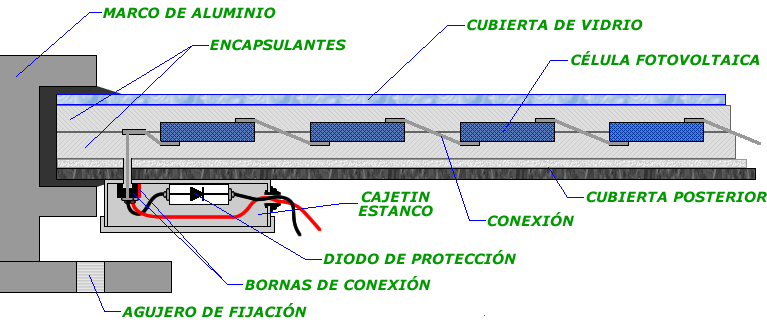
\includegraphics[width=.9\linewidth]{../figs/panel_fv.png}
\end{center}

\begin{itemize}
\item La asociación de células es encapsulada en \alert{dos capas de EVA} (etileno-vinilo-acetato), entre una \alert{lámina frontal de vidrio} y una \alert{capa posterior} de un polímero termoplástico (frecuentemente se emplea el \alert{tedlar}).

\item Este conjunto es enmarcado en una \alert{estructura de aluminio anodizado} con el objetivo de aumentar la resistencia mecánica del conjunto y facilitar el anclaje del módulo a las estructuras de soporte.
\end{itemize}
\end{frame}

\begin{frame}[label={sec:orgd78f164}]{El vidrio frontal}
\begin{itemize}[<+->]
\item Debe tener y mantener una \alert{alta transmisividad} en la banda espectral en la que trabajan las células solares.

\item Debe tener buena \alert{resistencia al impacto y a la abrasión}.

\item Su superficie debe ser de forma que combine un \alert{buen comportamiento antireflexivo} con la \alert{ausencia de bordes o desniveles} que faciliten
la acumulación de suciedad o dificulten la limpieza de ésta mediante la acción combinada del viento y la lluvia.

\item Frecuentemente se emplea \alert{vidrio templado con bajo contenido en hierro con algún tipo de tratamiento antireflexivo}.
\end{itemize}
\end{frame}

\begin{frame}[label={sec:org2ebf423}]{EVA}
\begin{itemize}
\item El \alert{encapsulante a base de EVA}, combinado con un tratamiento en vacío y las capas frontal y posterior, \alert{evita la entrada de humedad}
en el módulo, señalada como la causa principal de la degradación a largo plazo de módulos fotovoltaicos.

\item Además, esta combinación permite obtener \alert{altos niveles de aislamiento eléctrico}.
\end{itemize}
\end{frame}

\begin{frame}[label={sec:orga894ccd}]{Configuración eléctrica}
\begin{itemize}
\item Una \alert{configuración eléctrica muy común} hasta hace unos años empleaba \alert{36 células en serie} para obtener módulos con potencias comprendidas
en el rango \(\SIrange[range-phrase=-]{50}{100}{\wattpeak}\) con tensiones en MPP cercanas a los \(\SI{15}{\volt}\) en funcionamiento.

\item Estos módulos eran particularmente adecuados para su acoplamiento con baterías de tensión nominal \(\SI{12}{\volt}\) en los sistemas de
electrificación rural.

\item Con el protagonismo abrumador de los sistemas fotovoltaicos de conexión a red, esta configuración ha perdido importancia. Ahora son frecuentes los módulos de potencia superior a los \(\SI{200}{\wattpeak}\) y tensiones en el rango \(\SIrange[range-phrase=-]{30}{50}{\volt}\).
\end{itemize}
\end{frame}

\begin{frame}[label={sec:org0a7058e}]{Norma Internacional IEC 61215}
\begin{itemize}
\item Para los módulos compuestos por \alert{células de silicio cristalino} es de aplicación la \alert{norma internacional IEC-61215} \guillemotleft{}Crystalline Silicon
Terrestrial Photovoltaic (PV) Modules - Design Qualification and Type Approval\guillemotright{}.

\item Esta norma internacional recoge los \alert{requisitos de diseño y construcción} de módulos fotovoltaicos terrestres apropiados para su operación en períodos prolongados de tiempo bajo los efectos climáticos.

\item Detalla un \alert{procedimiento de pruebas} a los que se debe someter el módulo que desee contar con la certificación asociada a esta normativa
\end{itemize}
\end{frame}

\subsection{Modelado de un módulo}
\label{sec:org0626169}

\begin{frame}[label={sec:org63cbd6f}]{Suposiciones del modelo}
\begin{itemize}[<+->]
\item Los efectos de la resistencia paralelo son despreciables

\item La corriente fotogenerada (\(I_{L}\)) es igual a la corriente de cortocircuito

\item En cualquier condición de operación \(\exp(\frac{V+I\cdot R_{s}}{V_{t}})\gg1\)
\end{itemize}

\[
I=I_{sc}\cdot(1-\exp(\frac{V-V_{oc}+I\cdot R_{s}}{V_{t}})
\]
\end{frame}

\begin{frame}[label={sec:org1f141f1}]{Efecto de la radiación y la temperatura}
\begin{itemize}[<+->]
\item La \alert{corriente de cortocircuito} depende exclusivamente y de forma lineal de la \alert{irradiancia}.
\end{itemize}
\[
I_{sc}=G_{ef}\cdot\frac{I_{sc}^{*}}{G^{*}}
\]

\begin{itemize}
\item La \alert{tensión de circuito abierto} depende exclusivamente de la \alert{temperatura de \emph{célula}}, y decrece linealmente con ella.
\end{itemize}
\[
V_{oc}(T_{c})=V_{oc}^{*}+(T_{c}-T_{c}^{*})\cdot\frac{dV_{oc}}{dT_{c}}
\]
\end{frame}

\begin{frame}[label={sec:org4c2b8ec}]{Temperatura de operación de célula}
\begin{itemize}
\item La \alert{temperatura de operación de la célula} depende de la \alert{temperatura y la irradiación}
\end{itemize}
$$T_{c}=T_{a}+G\cdot\frac{NOCT-20}{800}$$

\begin{itemize}
\item Como consecuencia, la \alert{eficiencia decrece} a razón de 0,5\% por grado centigrado.

\item La \alert{resistencia serie} es \alert{independiente} de las condiciones de operación.
\end{itemize}
\end{frame}

\begin{frame}[label={sec:org391338c}]{TONC}
\begin{itemize}
\item Temperatura que alcanza una \emph{célula} cuando su \emph{módulo} trabaja en las siguientes condiciones:

\begin{itemize}
\item Irradiancia: \(G=\SI{800}{\watt\per\meter\squared}\)

\item Espectro: el correspondiente a \(AM=1.5\).

\item Incidencia normal

\item Temperatura \emph{ambiente}: \(T_{a}=\SI{20}{\celsius}\).

\item Velocidad de viento: \(v_{v}=\SI{1}{\meter\per\second}\).
\end{itemize}
\end{itemize}
\end{frame}


\subsection{Punto Caliente}
\label{sec:orgc7f7315}

\begin{frame}[label={sec:orgb186fb8}]{Punto caliente}
\begin{center}
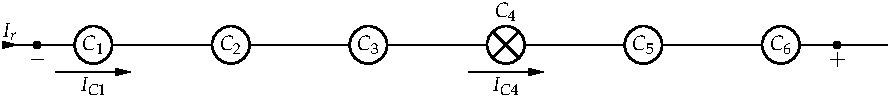
\includegraphics[width=.9\linewidth]{../figs/AsociacionSerieCelulas.pdf}
\end{center}
\end{frame}

\begin{frame}[label={sec:org3159691}]{Punto caliente}
\begin{center}
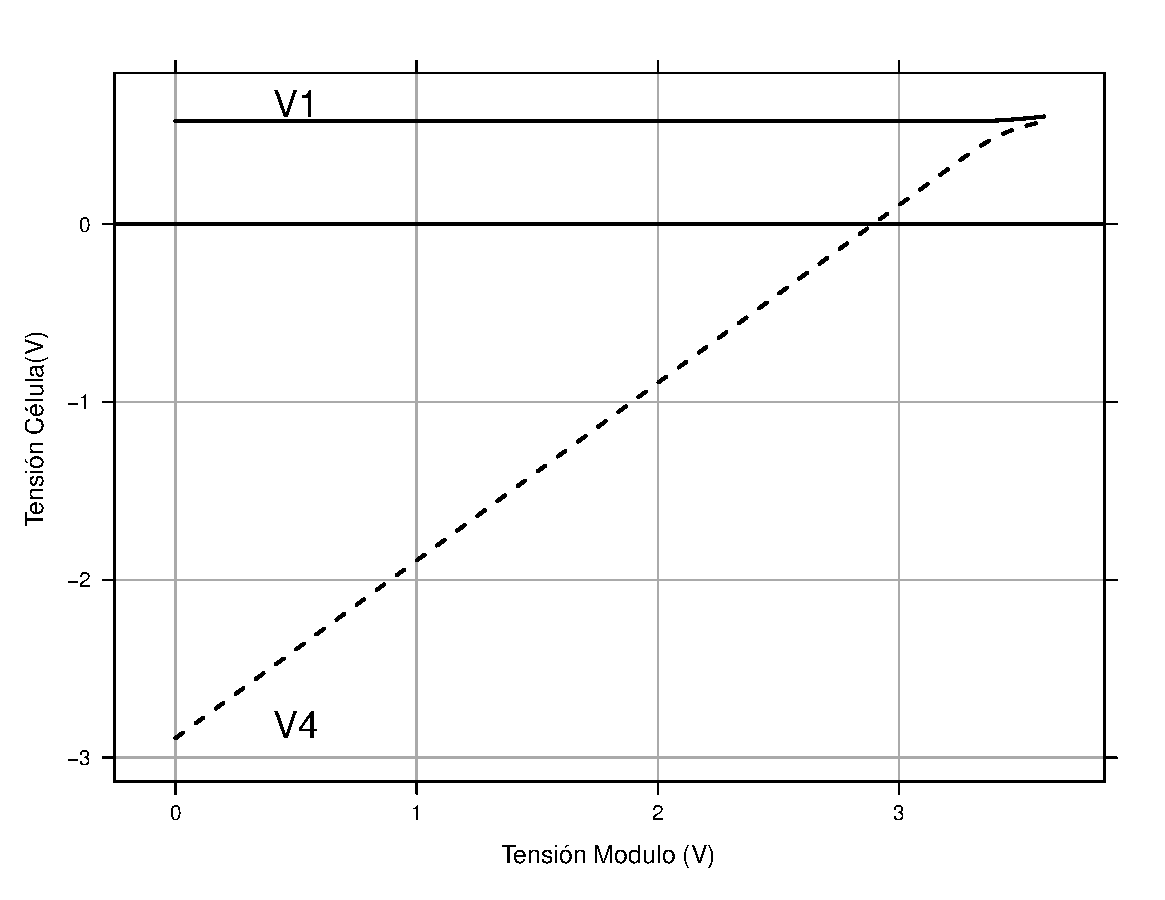
\includegraphics[width=.9\linewidth]{../figs/TensionCelula_Sombras.pdf}
\end{center}
\end{frame}

\begin{frame}[label={sec:org98ce028}]{Punto caliente}
\begin{center}
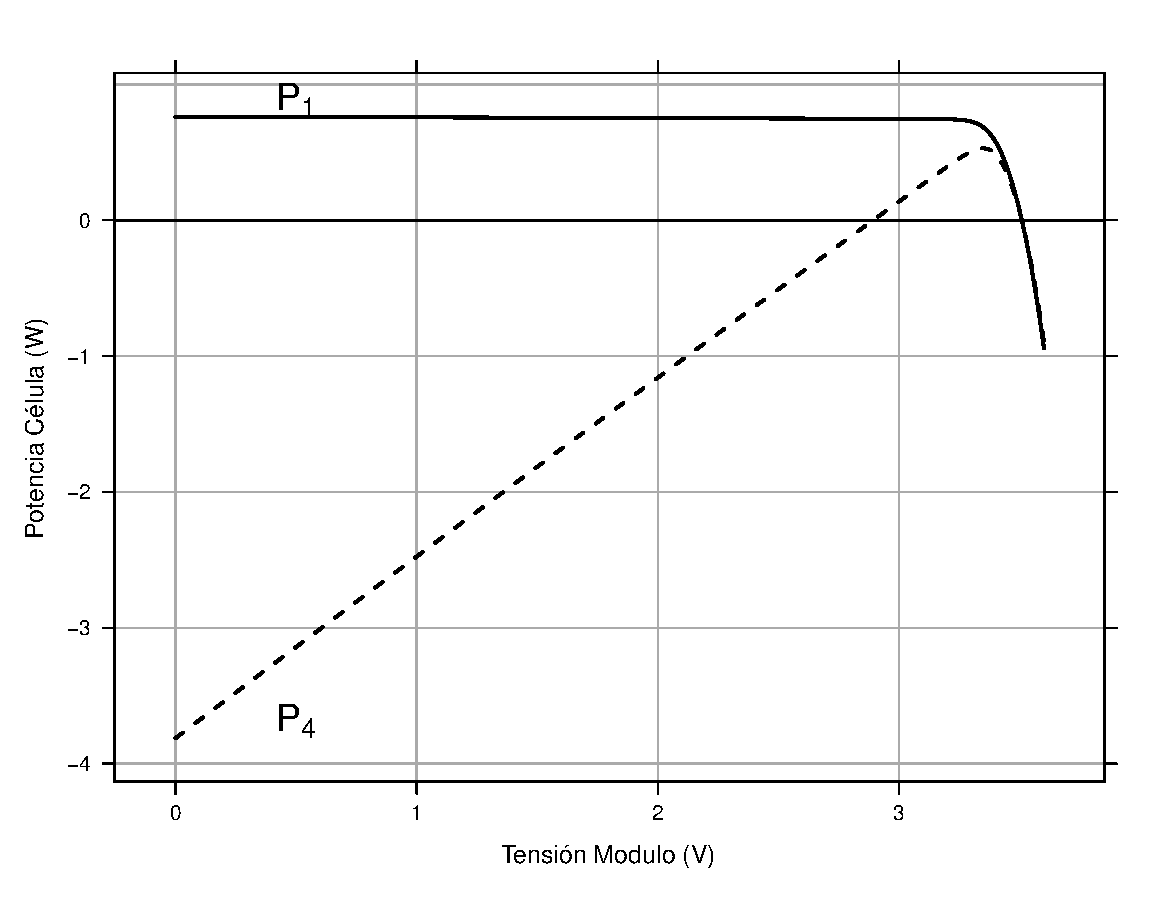
\includegraphics[width=.9\linewidth]{../figs/PotenciaCelula_Sombra.pdf}
\end{center}
\end{frame}

\begin{frame}[label={sec:org7449dcf}]{Diodo de paso}
\begin{center}
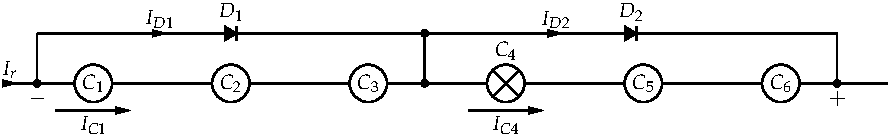
\includegraphics[width=.9\linewidth]{../figs/AsociacionSerieCelulas_DiodosPaso.pdf}
\end{center}
\end{frame}

\begin{frame}[label={sec:org755698f}]{Curvas I-V con diodo de paso}
\begin{center}
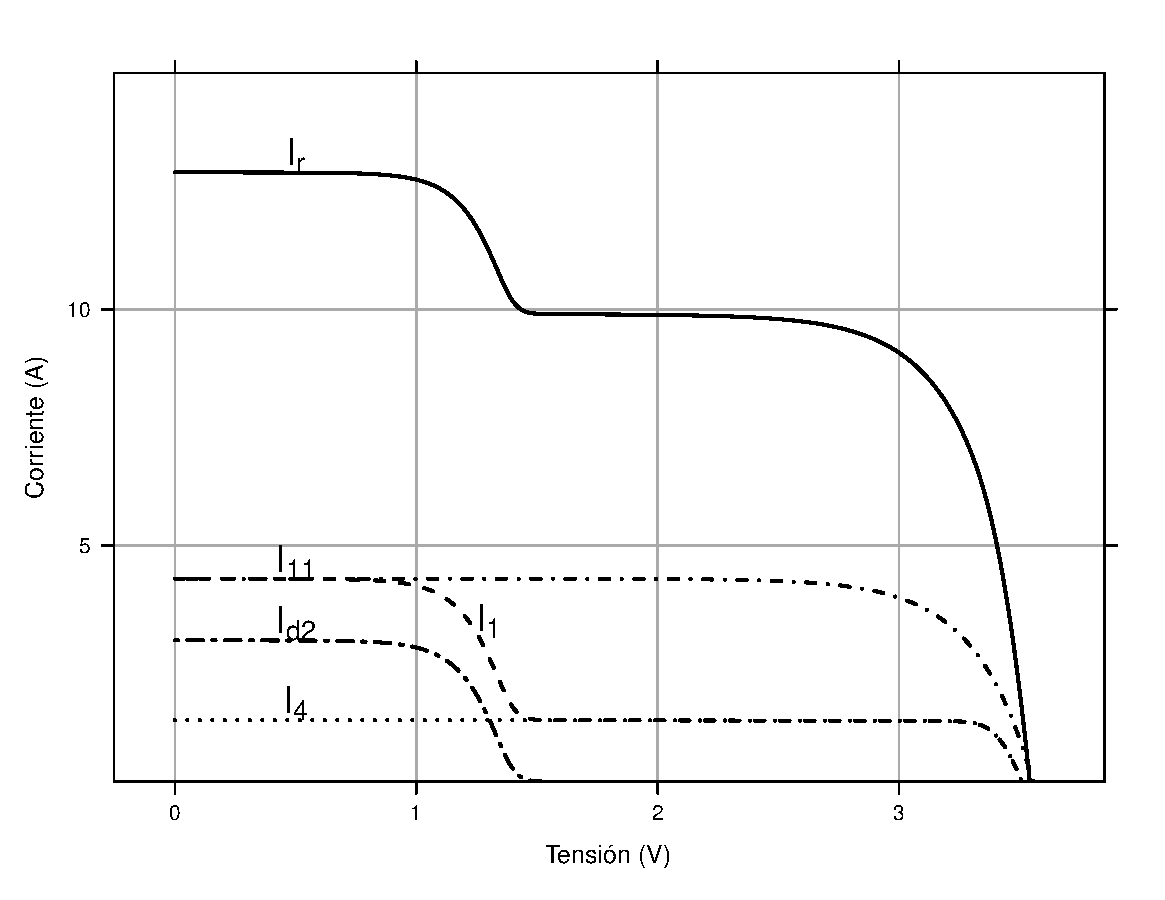
\includegraphics[width=.9\linewidth]{../figs/CurvaIV_DiodoPaso.pdf}
\end{center}
\end{frame}

\begin{frame}[label={sec:org021bcae}]{Tensión con diodo de paso}
\begin{center}
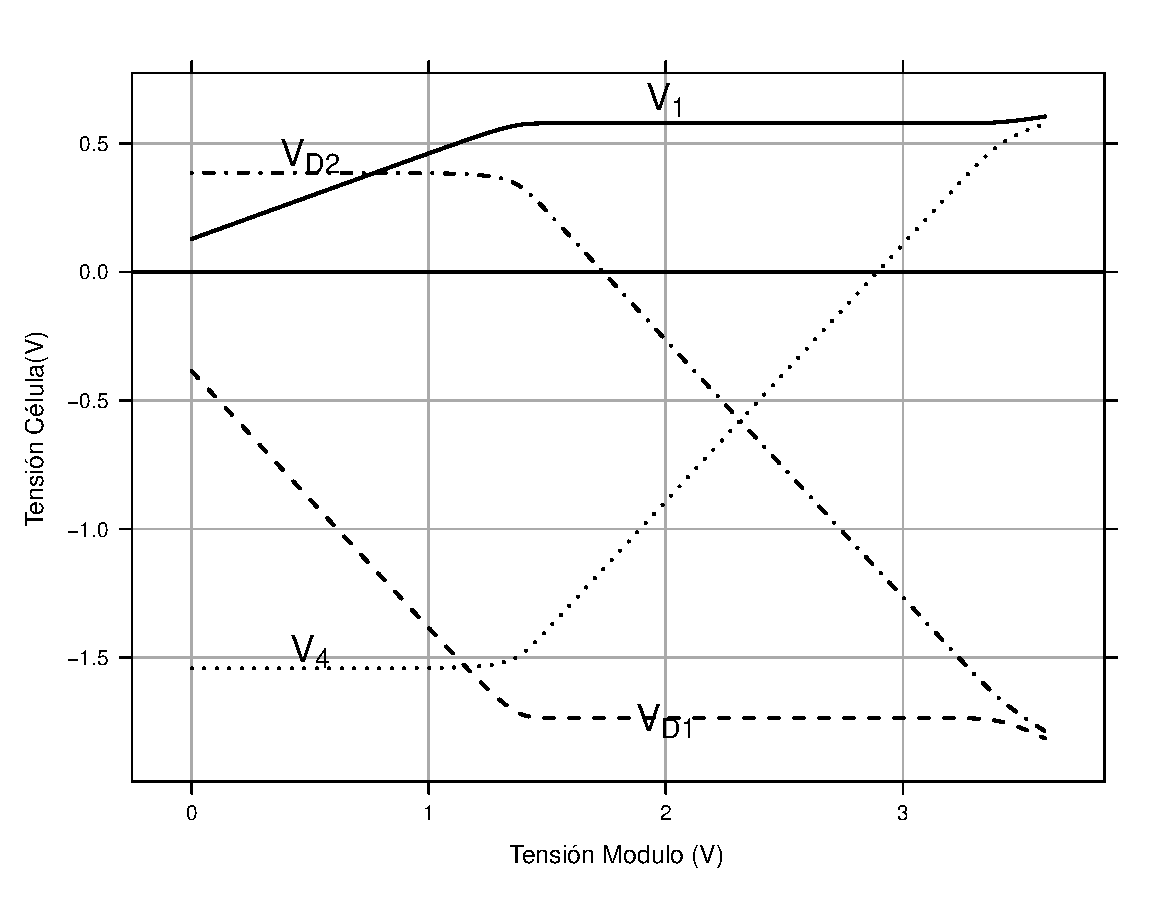
\includegraphics[width=.9\linewidth]{../figs/TensionesCelulasDiodos_DiodoPaso.pdf}
\end{center}
\end{frame}

\begin{frame}[label={sec:org140fd82}]{Curvas Potencia con diodo de paso}
\begin{center}
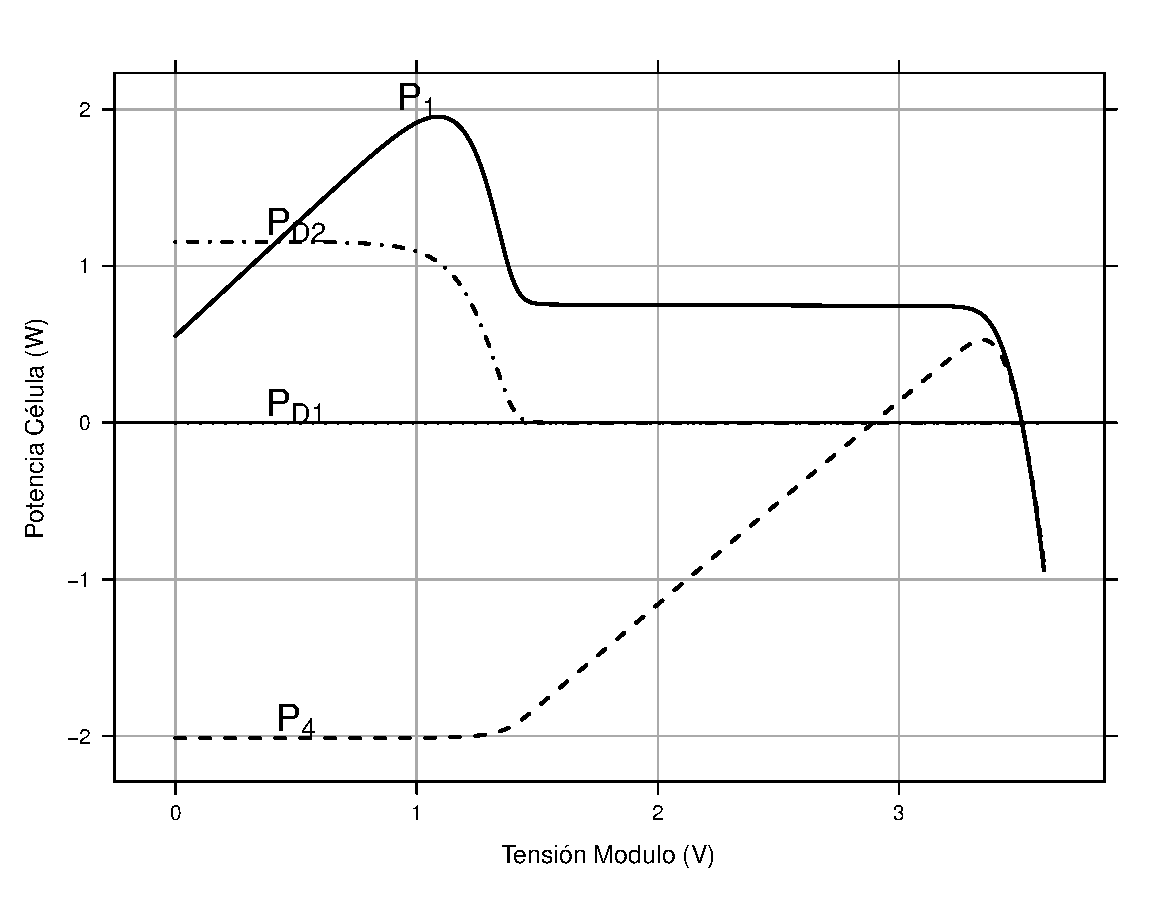
\includegraphics[width=.9\linewidth]{../figs/PotenciaCelulas_DiodoPaso.pdf}
\end{center}
\end{frame}

\begin{frame}[label={sec:orgc1bd7d3}]{Curva Módulo con Diodos de Paso}
\begin{center}
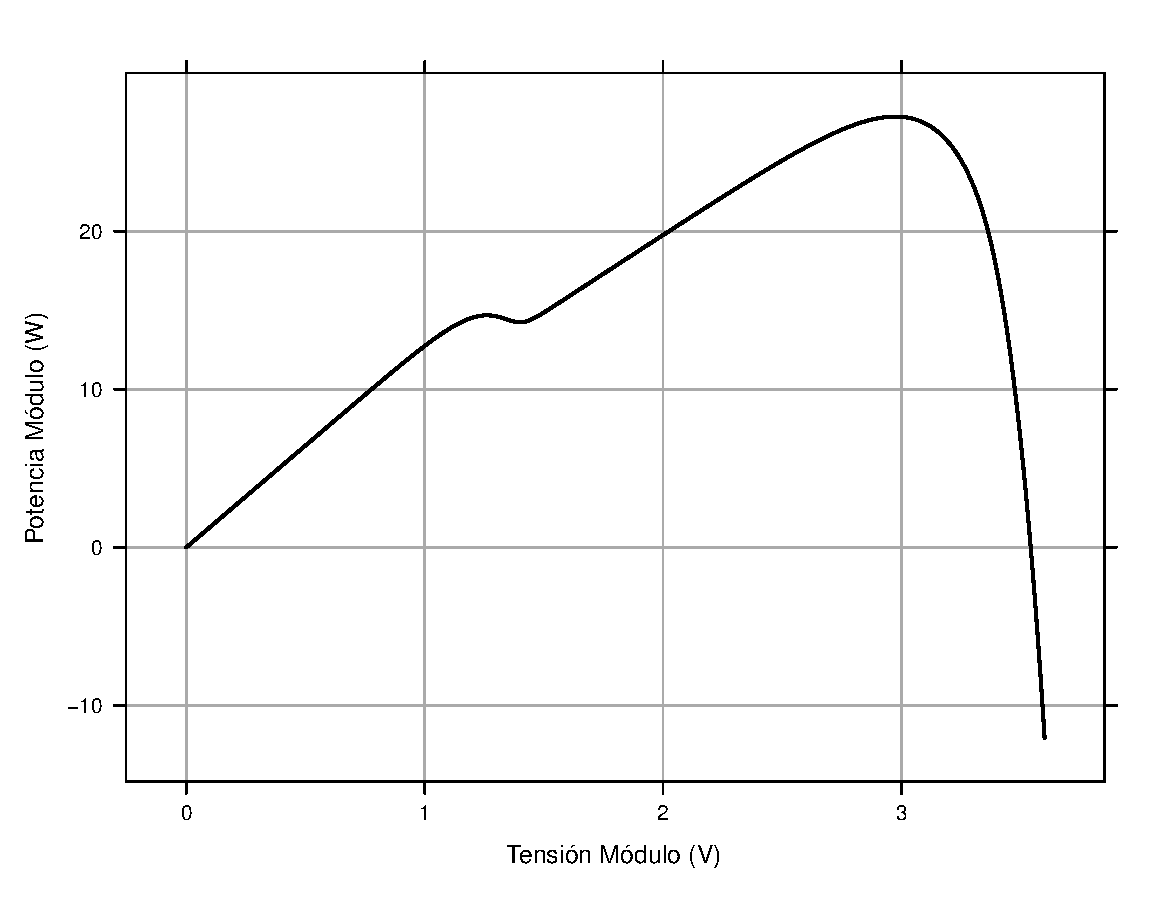
\includegraphics[width=.9\linewidth]{../figs/PotenciaModulo.pdf}
\end{center}
\end{frame}

\begin{frame}[label={sec:org8b3d57d}]{Diodos de paso}
\begin{center}
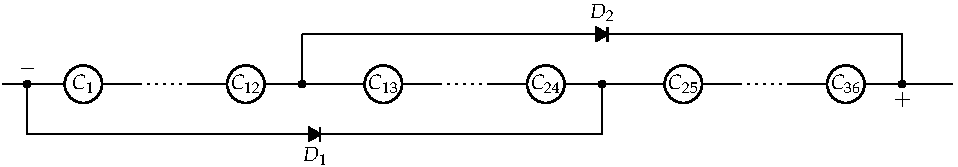
\includegraphics[width=.9\linewidth]{../figs/AsociacionSerieCelulas_DiodosPasoAlternos.pdf}
\end{center}
\end{frame}

\section{Generador Fotovoltaico}
\label{sec:org06bf6dd}

\subsection{Definición}
\label{sec:orgf022937}

\begin{frame}[label={sec:org6e93a53}]{Generador Fotovoltaico}
\begin{columns}
\begin{column}{0.7\columnwidth}
\begin{itemize}[<+->]
\item Un generador fotovoltaico es una \alert{asociación eléctrica de módulos fotovoltaicos} para adaptarse a las condiciones de funcionamiento de una aplicación determinada.

\item Se compone de un total de \(N_T = N_{p}\cdot N_{s}\) módulos, siendo \(N_{p}\) el número de ramas (módulos en paralelo), y \(N_{s}\) el número de módulos en cada serie.
\end{itemize}
\end{column}


\begin{column}{0.3\columnwidth}
\begin{center}
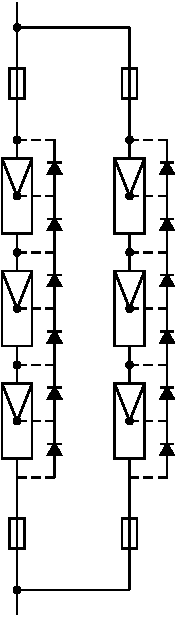
\includegraphics[height=0.9\textheight]{../figs/AsociacionModulos.pdf}
\end{center}
\end{column}
\end{columns}
\end{frame}

\begin{frame}[label={sec:orgdf31d95}]{Ramas y series}
\begin{columns}
\begin{column}{0.7\columnwidth}
\begin{itemize}
\item El número de ramas, \(N_p\), define la corriente total del generador
\end{itemize}
\[
I_{sc,g} = N_p \cdot I_{sc,m}
\]
\begin{itemize}
\item El número de modulos en serie, \(N_s\), define la tensión del generador.
\end{itemize}
\[
V_{oc,g} = N_s \cdot V_{oc,m}
\]
\begin{itemize}
\item La potencia del generador es (idealmente):
\end{itemize}
\[
P_g = N_T \cdot P_m = (N_s \cdot V_{mpp, m}) (N_p \cdot I_{mpp, m})
\]
\end{column}



\begin{column}{0.3\columnwidth}
\begin{center}
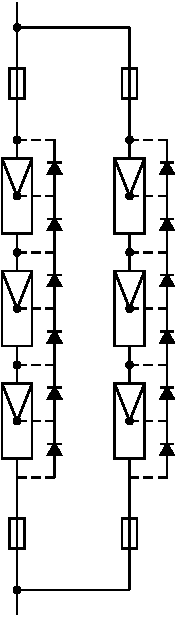
\includegraphics[height=0.9\textheight]{../figs/AsociacionModulos.pdf}
\end{center}
\end{column}
\end{columns}
\end{frame}

\begin{frame}[label={sec:org65b5d24}]{Ejemplo de cálculo}
Calcular el comportamiento eléctrico de un generador fotovoltaico constituido por 40 módulos, asociados en 4 ramas, bajo la suposición de factor de forma constante.

\begin{itemize}
\item Las condiciones de operación de este generador son:  \(G_{ef}=700\, W/m^{2}\) y \(T_{a}=34\celsius\).

\item De las fichas técnicas del módulo se extrae la siguiente información: \(I_{sc}^{*}=3\, A\), \(V_{oc}^{*}=19,8\, V\), \(I_{mpp}^{*}=2,8\, A\) y \(V_{mpp}^{*}=15.7\, V\).

\item Cada módulo está constituido por 33 células asociadas en serie. La TONC del módulo es de \(43\celsius\).
\end{itemize}
\end{frame}

\subsection{Pérdidas por dispersión}
\label{sec:orgdb72401}

\begin{frame}[label={sec:org2036a99}]{Pérdidas por dispersión}
\begin{block}{Definición del problema}
Los parámetros eléctricos de un módulo FV presentan dispersión: la producción energética será menor que la ideal.
\end{block}
\end{frame}

\begin{frame}[label={sec:org384c283}]{Distribución de valores de corriente y tensión}
La corriente de máxima potencia de un conjunto de módulos puede caracterizarse por una distribución tipo
Weibull$$f(I_{mpp})=\alpha\beta^{-\alpha}I_{mpp}^{\alpha-1}exp\left[-\left(\frac{I_{mpp}}{\beta}\right)^{\alpha}\right]$$
siendo \(\alpha\) el factor de forma y \(\beta\) el factor de escala de la distribución. La eficiencia de conexión serie
es:$$\eta_{cs}=\frac{I_{mpp}^{r}}{\overline{I_{mpp}}}$$ siendo \(I_{mpp}^{r}\) la corriente de la rama, y \(\overline{I_{mpp}}\) la media
de las corrientes del grupo de módulos.
\end{frame}

\begin{frame}[label={sec:org2b5b8d6}]{Eficiencia de conexión}
\begin{itemize}
\item A partir de la distribución y la definición de eficiencia de conexión serie puede deducirse que ésta se calcula mediante $$\eta_{cs}=N^{-\frac{1}{\alpha}}$$ siendo N el número de módulos en la serie. Por tanto, \alert{la eficiencia disminuye si aumenta N}. Asimismo, la eficiencia aumenta con \(\alpha\).

\item Por otra parte, puede demostrarse que la \alert{tensión de un grupo de módulos} puede modelarse mediante una función \alert{gaussiana} y que \alert{la dispersión de valores de tensión es suficientemente baja para poder  considerar que la eficiencia de conexión de ramas en paralelo es igual a 1.}
\end{itemize}
\end{frame}

\begin{frame}[label={sec:orgcf2ea58}]{Clasificación de módulos}
\begin{itemize}
\item La dispersión de un conjunto depende inversamente del valor de
\(\alpha\), así que un \alert{método para reducir las pérdidas por
dispersión} consiste en \alert{realizar clasificaciones} de los módulos
atendiendo a sus valores reales de corriente.

\item En sistemas de cierta entidad, puede ser conveniente realizar una
clasificación en tres categorías y crear cada rama con módulos de una
misma categoría.

\item Este método puede suponer reducciones del 2-3\% en las pérdidas
globales del sistema.
\end{itemize}
\end{frame}

\begin{frame}[label={sec:org9cb0b2c}]{Pérdidas por dispersión}
\begin{block}{Problema}
\begin{itemize}
\item Las clasificaciones se realizan en base a las médidas realizadas por
los fabricantes con\guillemotleft{}flash\guillemotright{}.

\item \alert{La indeterminación asociada a este método en relación a las medidas
a sol real son del mismo rango que la separación entre categorías.}
\end{itemize}
\end{block}
\end{frame}


\section{Ejemplos de generadores fotovoltaicos}
\label{sec:orgcd05f03}

\begin{frame}[label={sec:orgaa7b303}]{}
\begin{center}
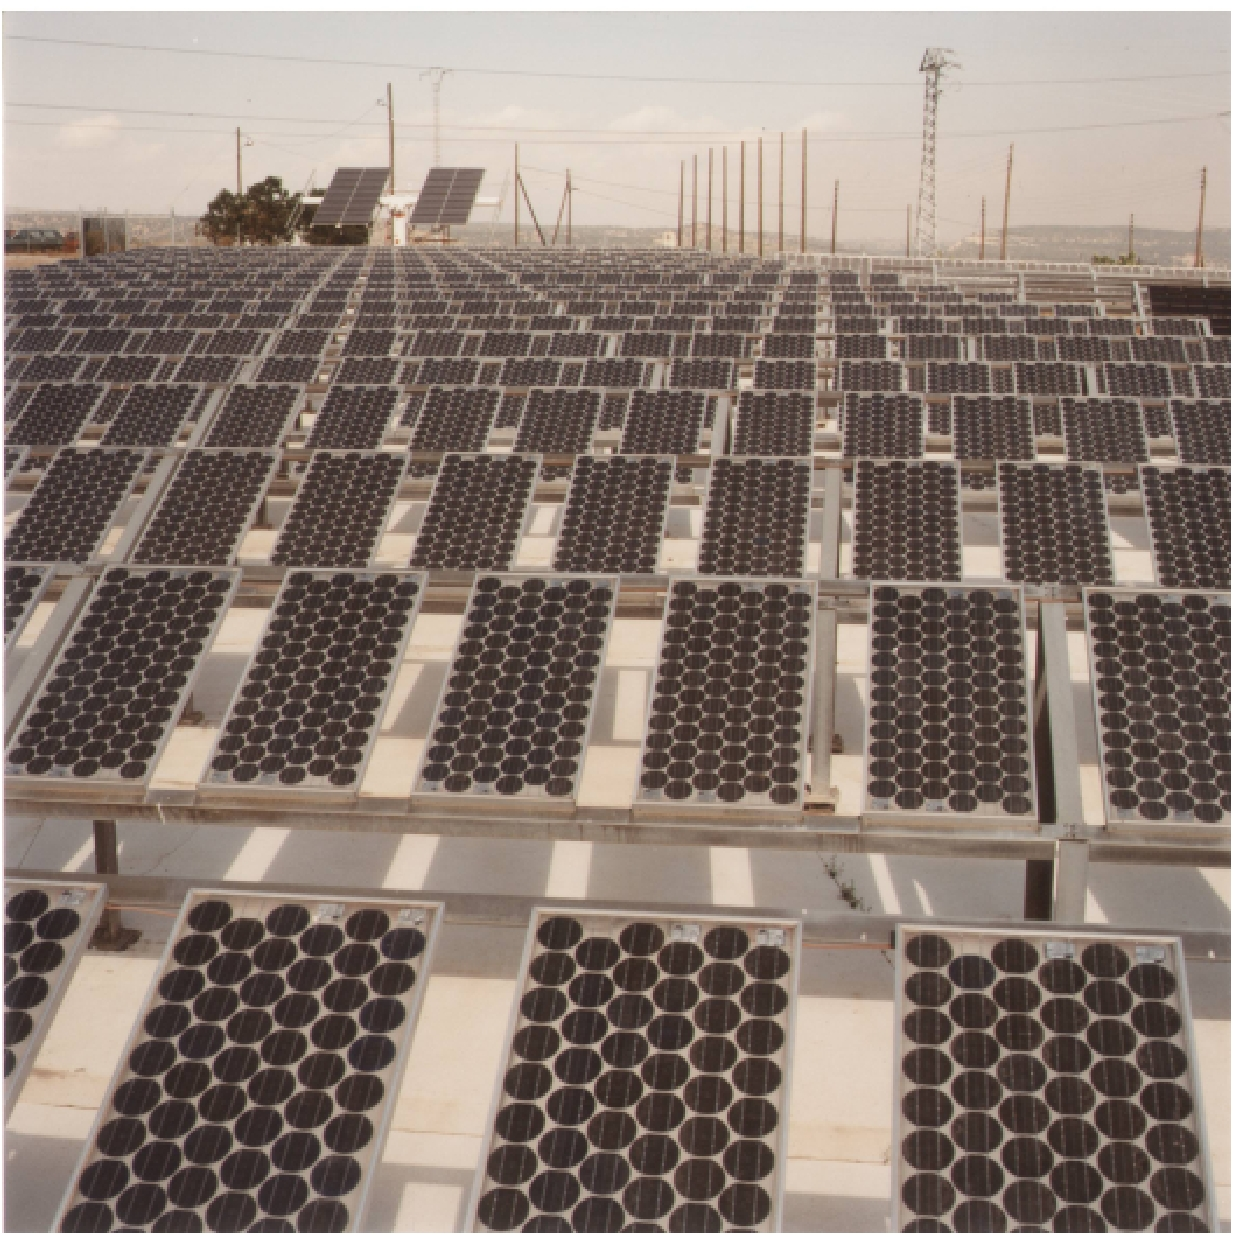
\includegraphics[width=.9\linewidth]{../figs/Bifacial.jpg}
\end{center}
\end{frame}

\begin{frame}[label={sec:org726a046}]{}
\begin{center}
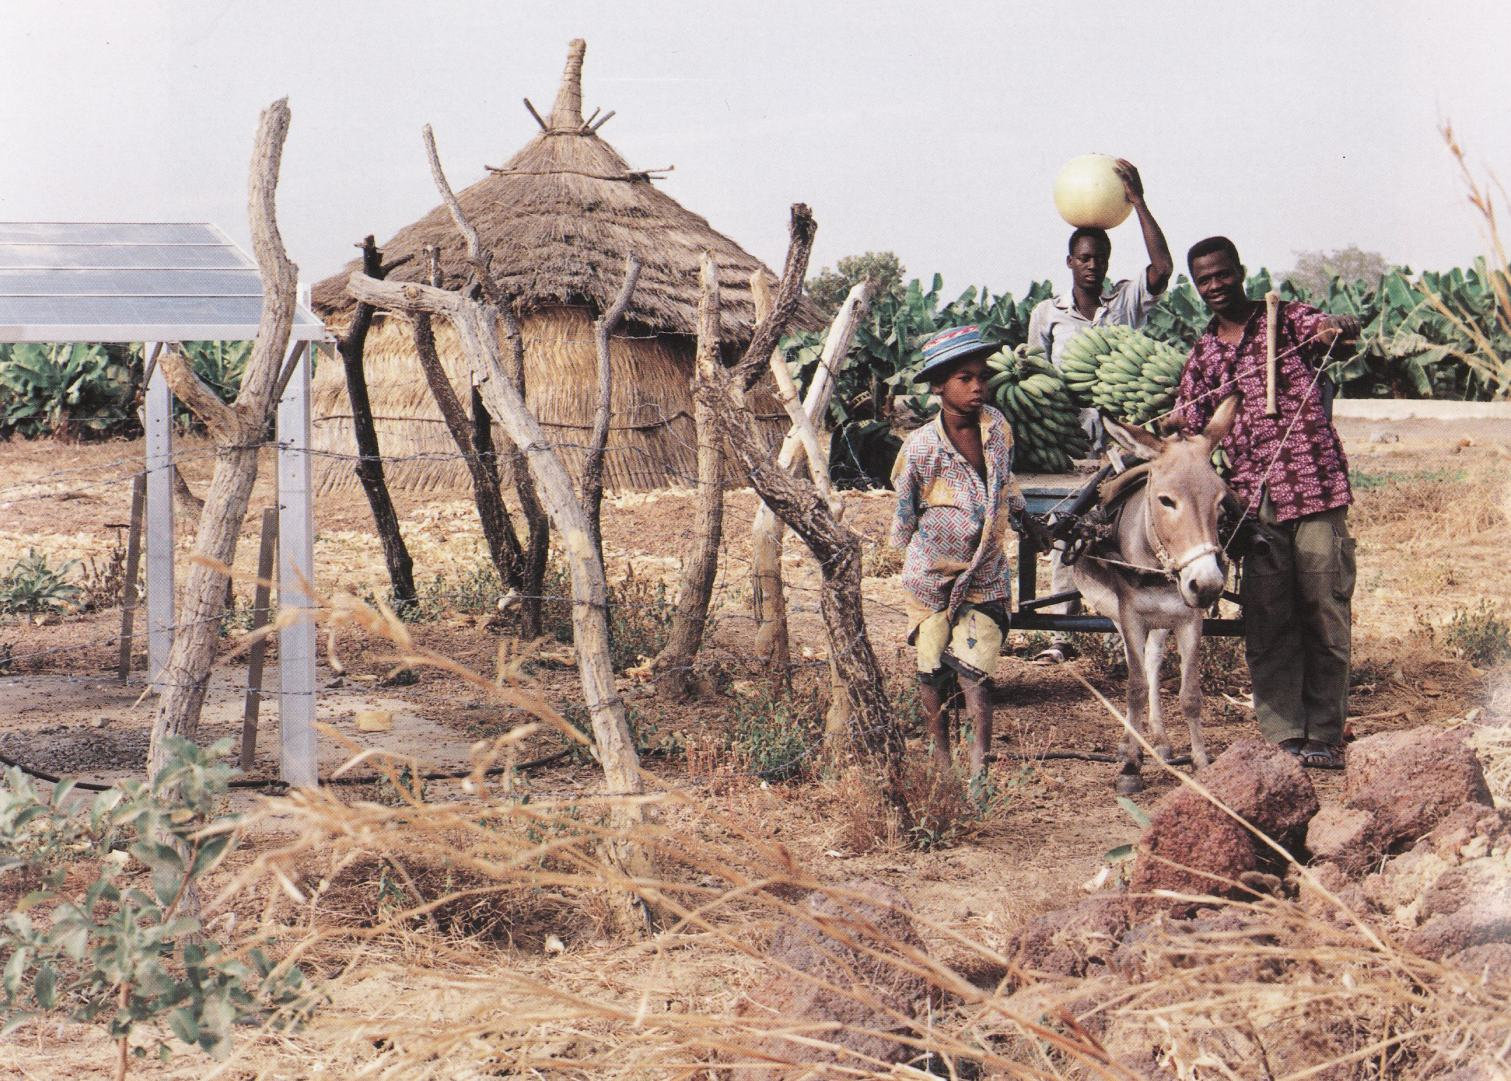
\includegraphics[width=.9\linewidth]{../figs/er.jpg}
\end{center}
\end{frame}

\begin{frame}[label={sec:org1bba862}]{}
\begin{center}
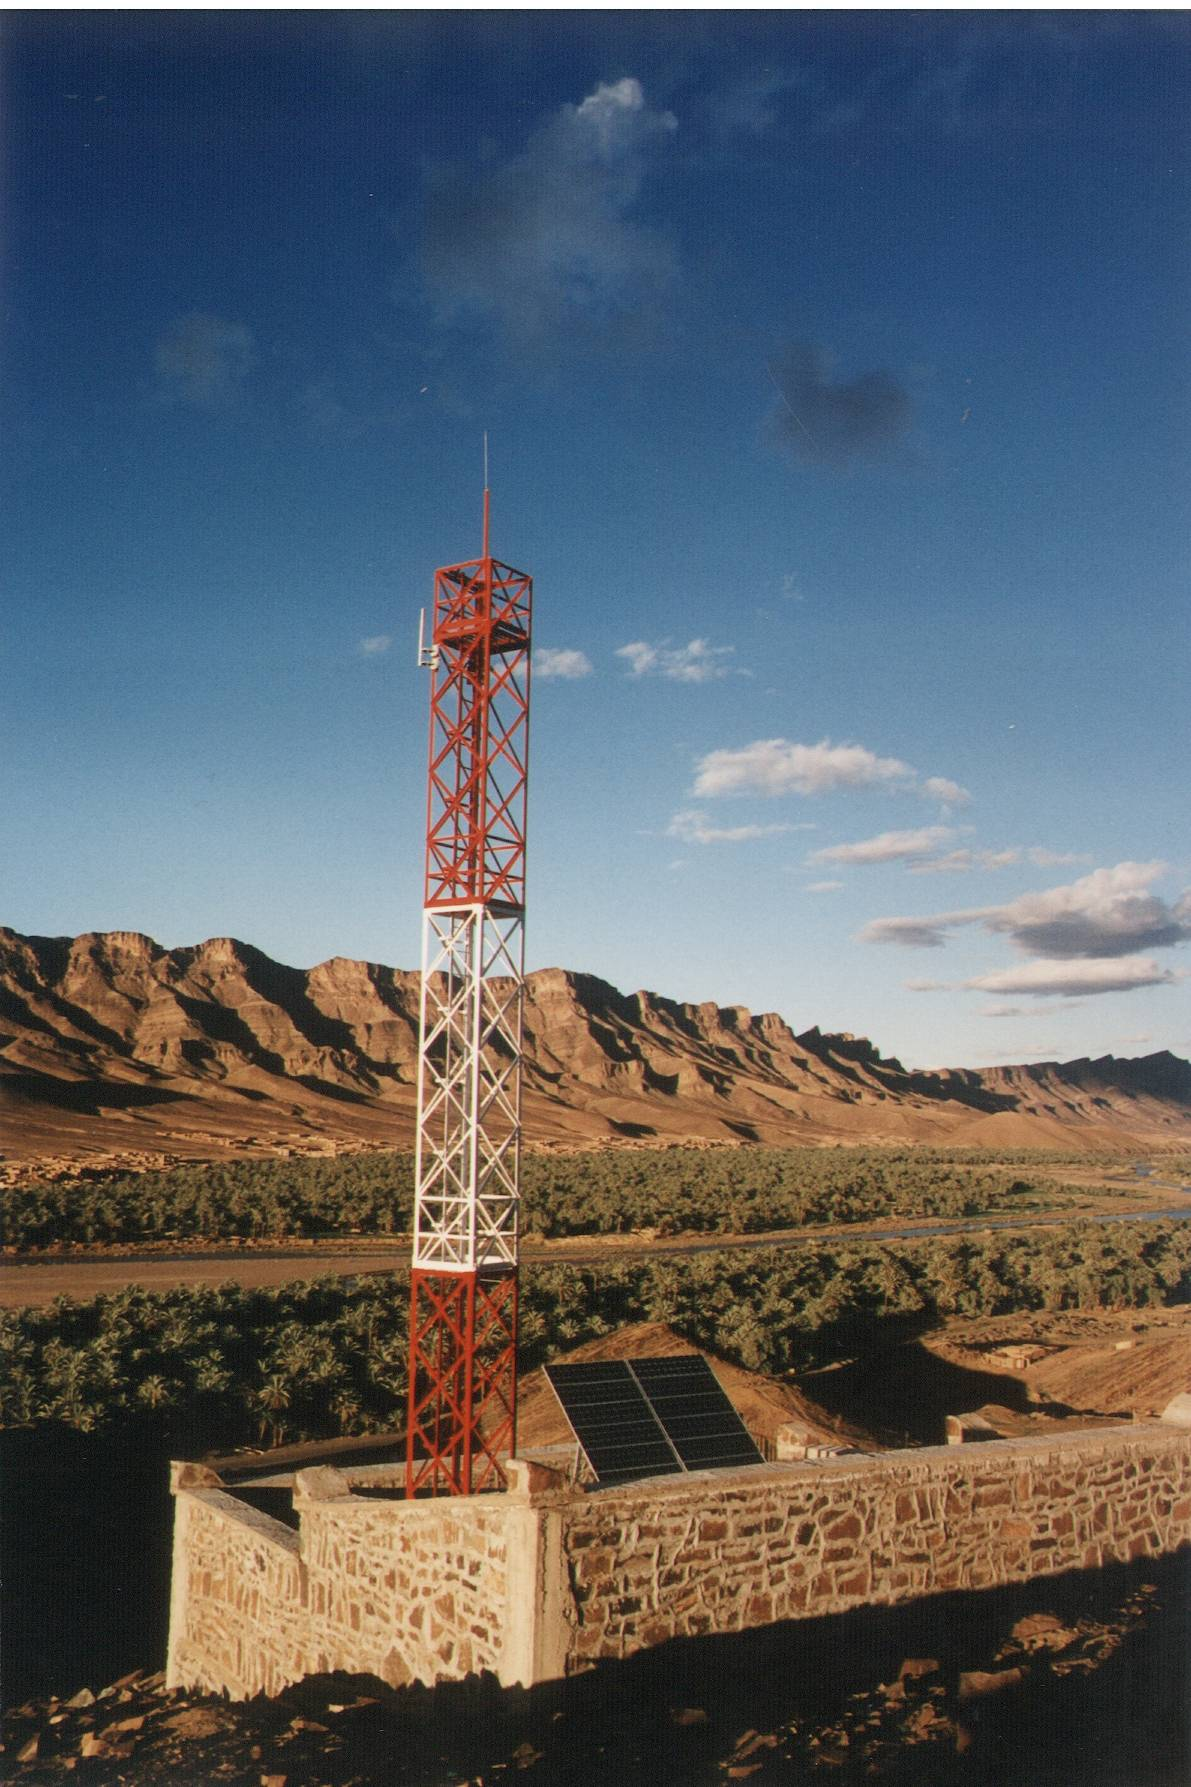
\includegraphics[height=0.9\textheight]{../figs/TelefoniaRural.jpg}
\end{center}
\end{frame}

\begin{frame}[label={sec:orge3562b2}]{}
\begin{center}
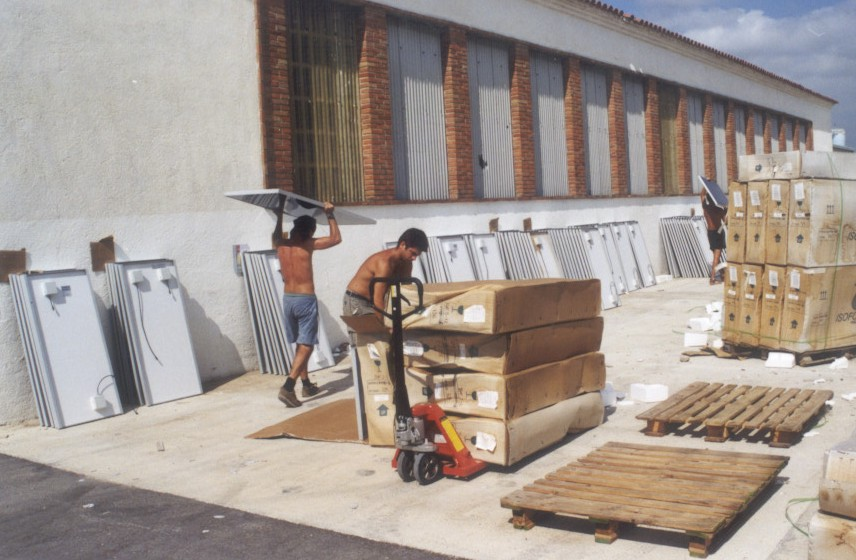
\includegraphics[width=.9\linewidth]{../figs/clasificacion2.jpg}
\end{center}
\end{frame}

\begin{frame}[label={sec:orgff74b18}]{}
\begin{center}
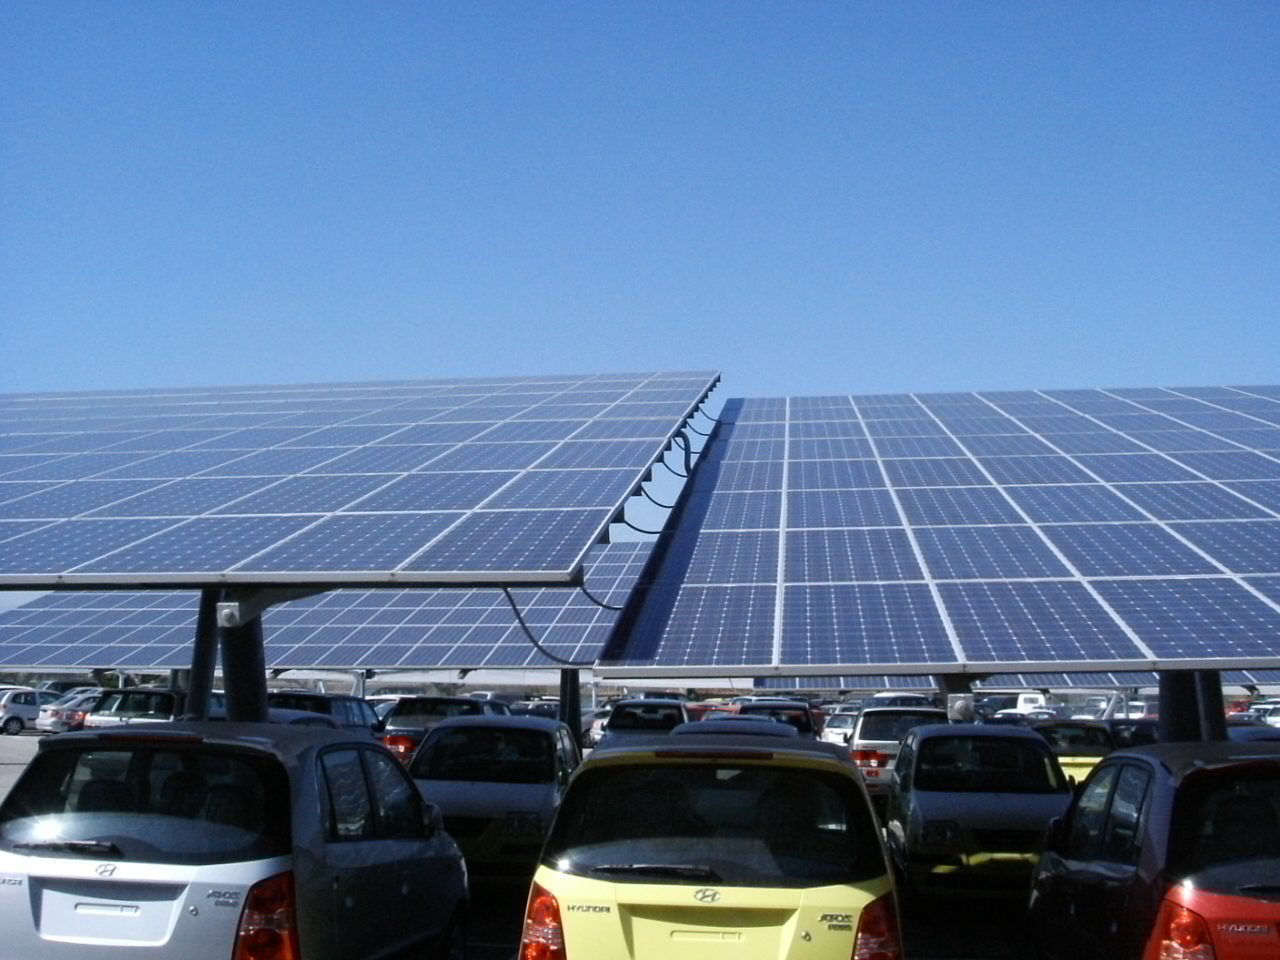
\includegraphics[width=.9\linewidth]{../figs/dscf0997.jpg}
\end{center}
\end{frame}

\begin{frame}[label={sec:org02d6b13}]{}
\begin{center}
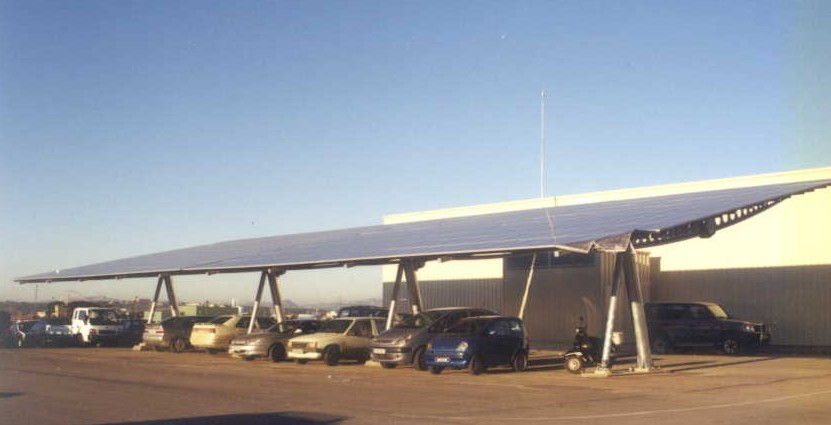
\includegraphics[width=.9\linewidth]{../figs/ModulosRotos.jpg}
\end{center}
\end{frame}

\begin{frame}[label={sec:orga9d293b}]{}
\begin{center}
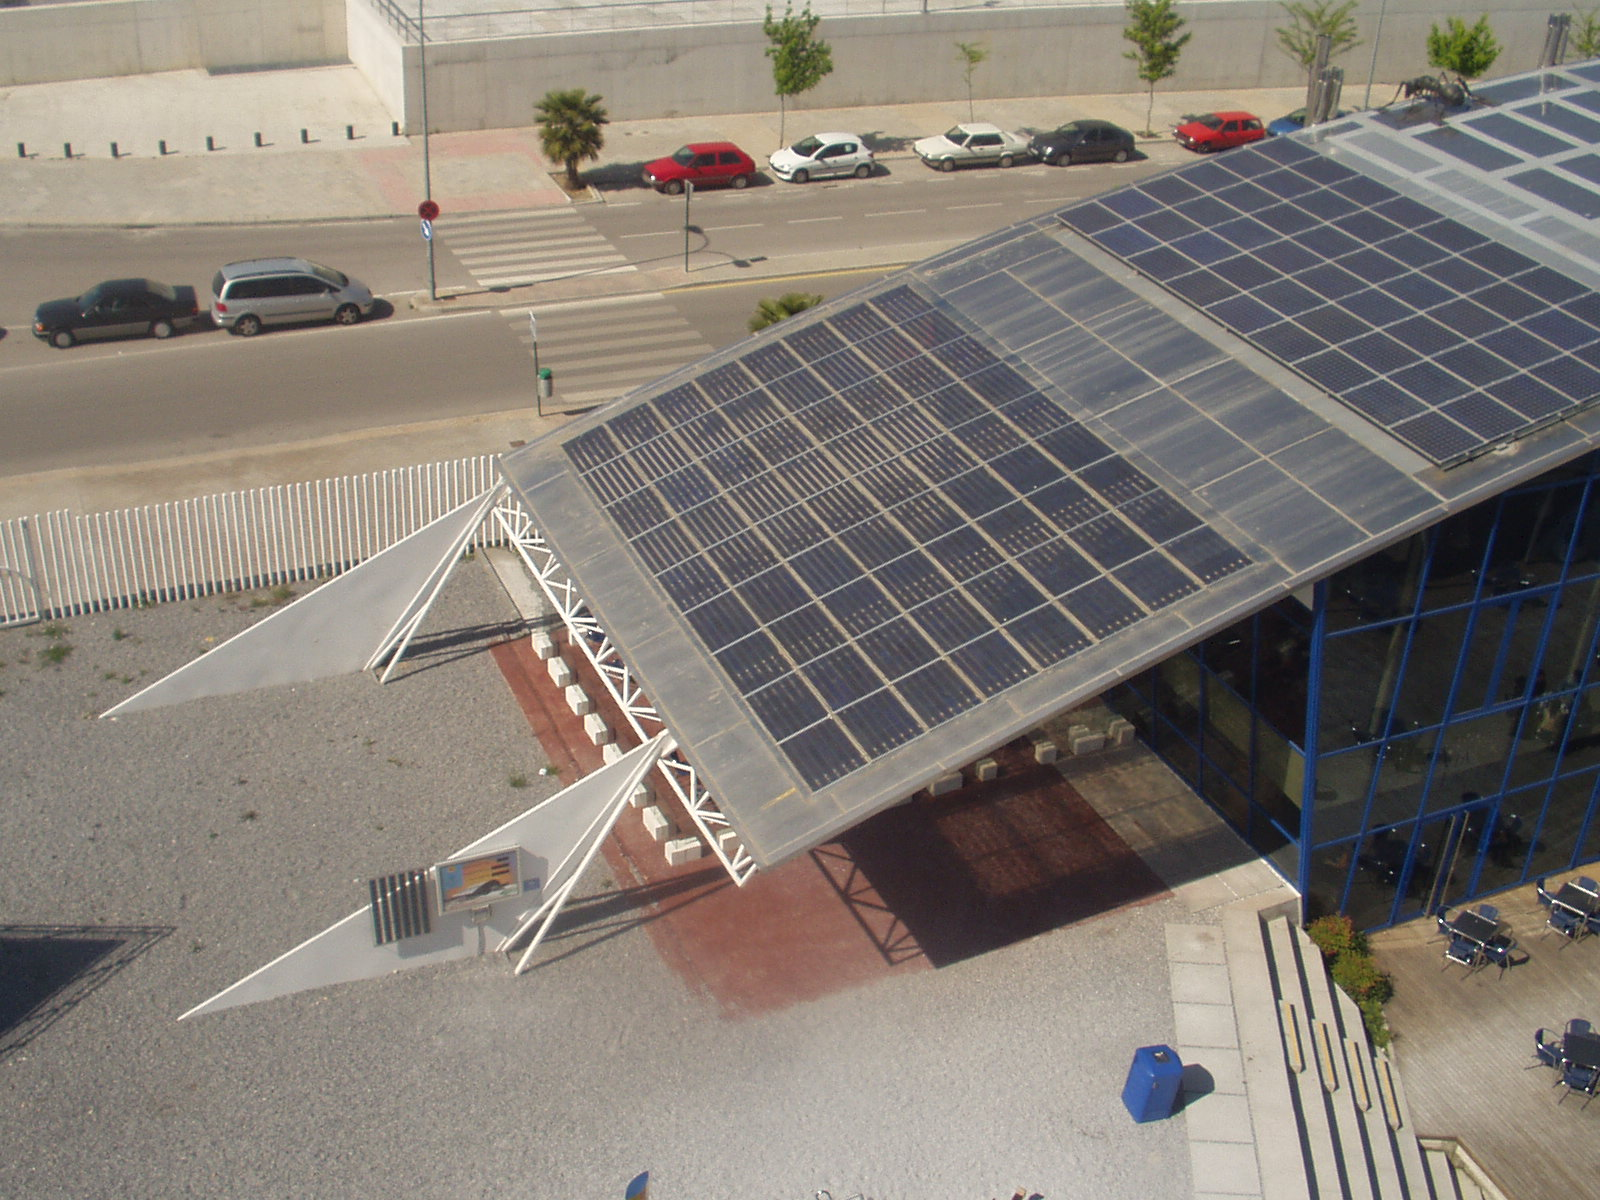
\includegraphics[width=.9\linewidth]{../figs/p1010007.jpg}
\end{center}
\end{frame}

\begin{frame}[label={sec:org3c6b794}]{}
\begin{center}
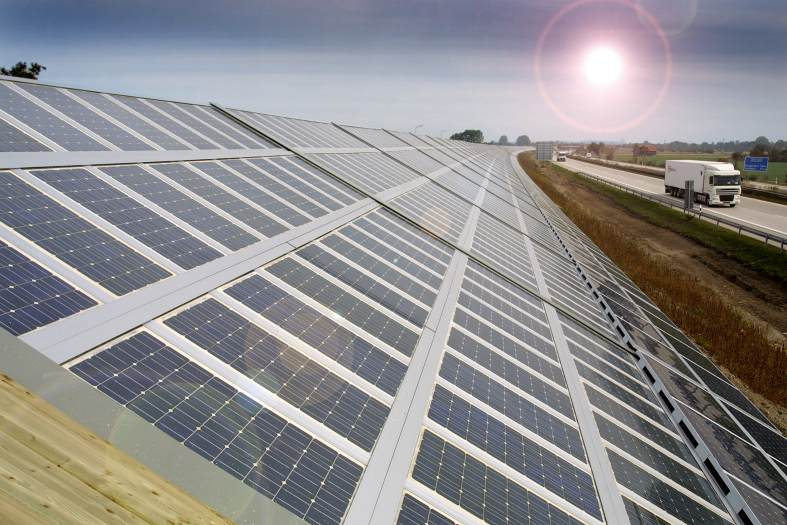
\includegraphics[width=.9\linewidth]{../figs/BarreraRuido.jpg}
\end{center}
\end{frame}
\begin{frame}[label={sec:org01fc8fc}]{}
\begin{center}
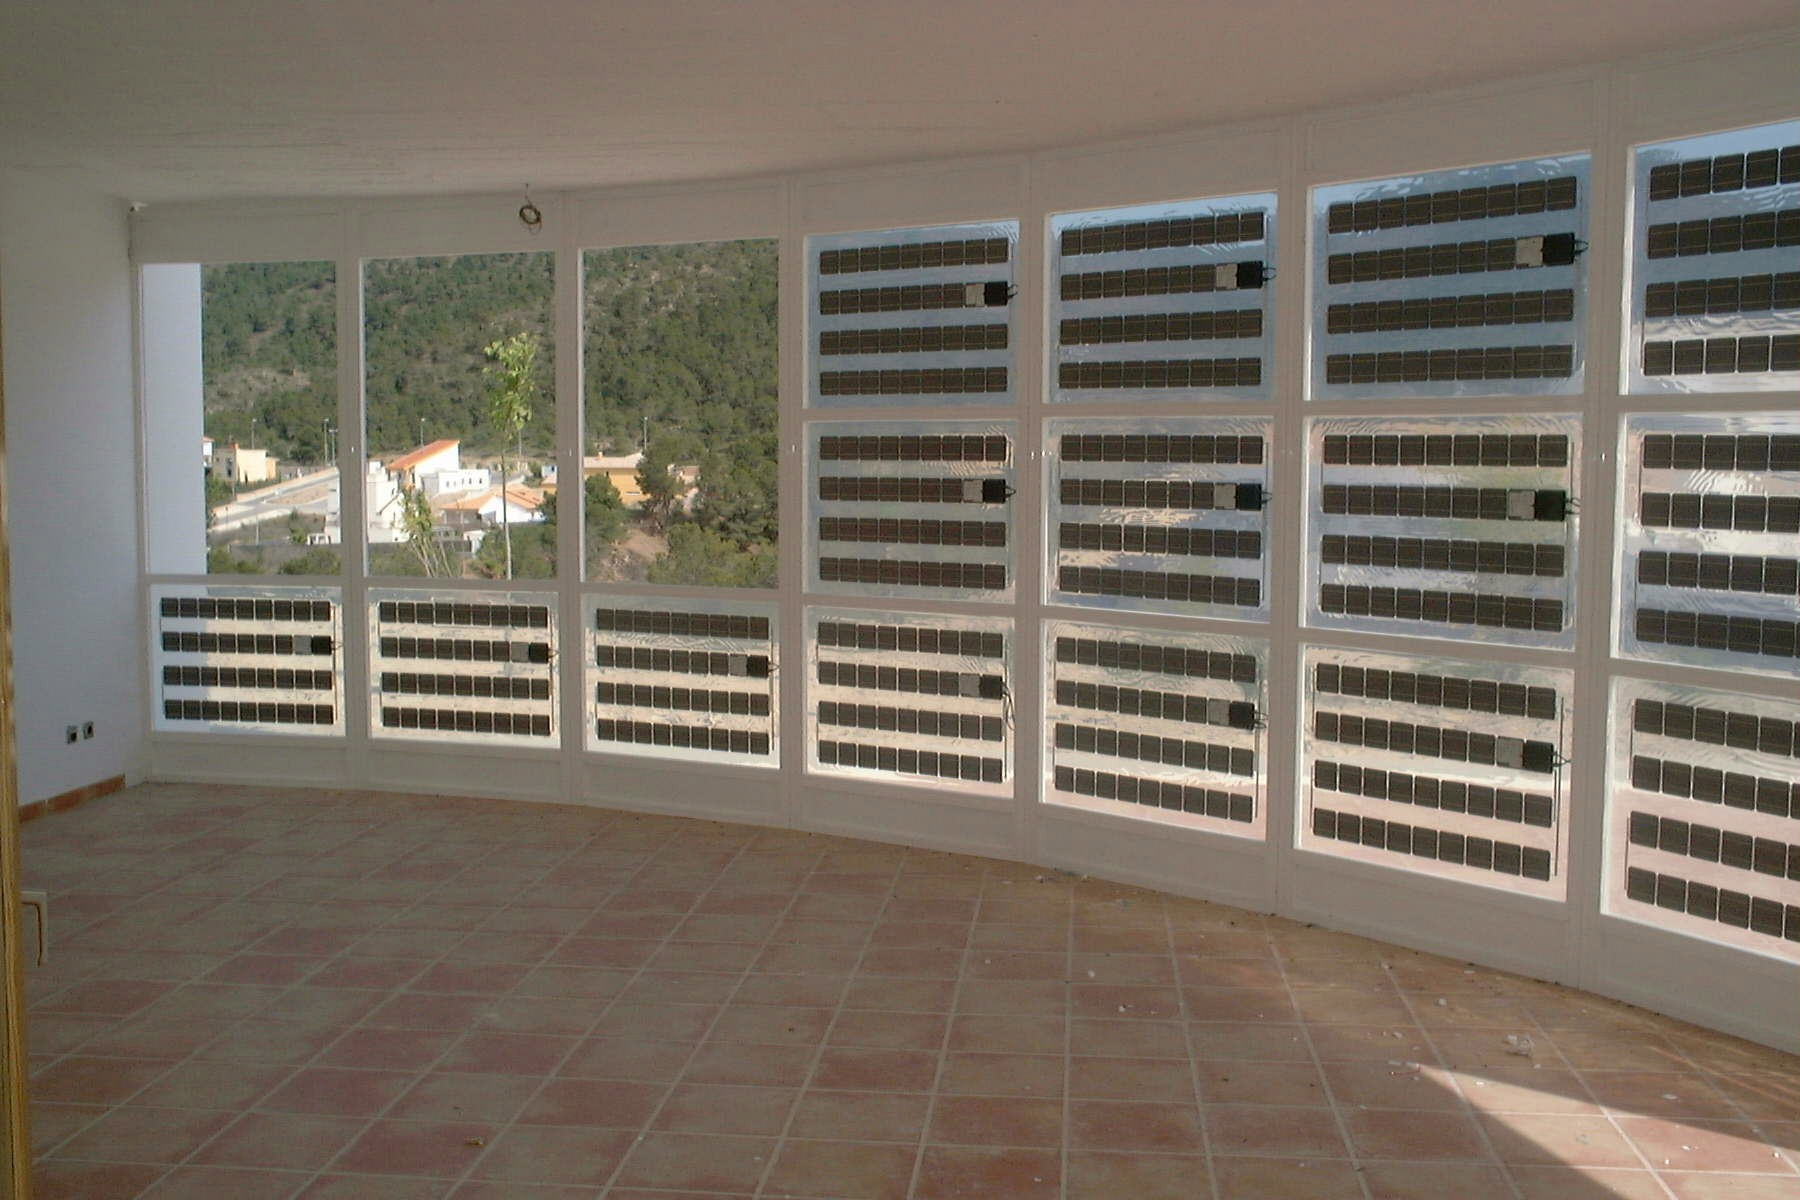
\includegraphics[width=.9\linewidth]{../figs/TorreguilInterior2.jpg}
\end{center}
\end{frame}

\begin{frame}[label={sec:org1bf167e}]{}
\begin{center}
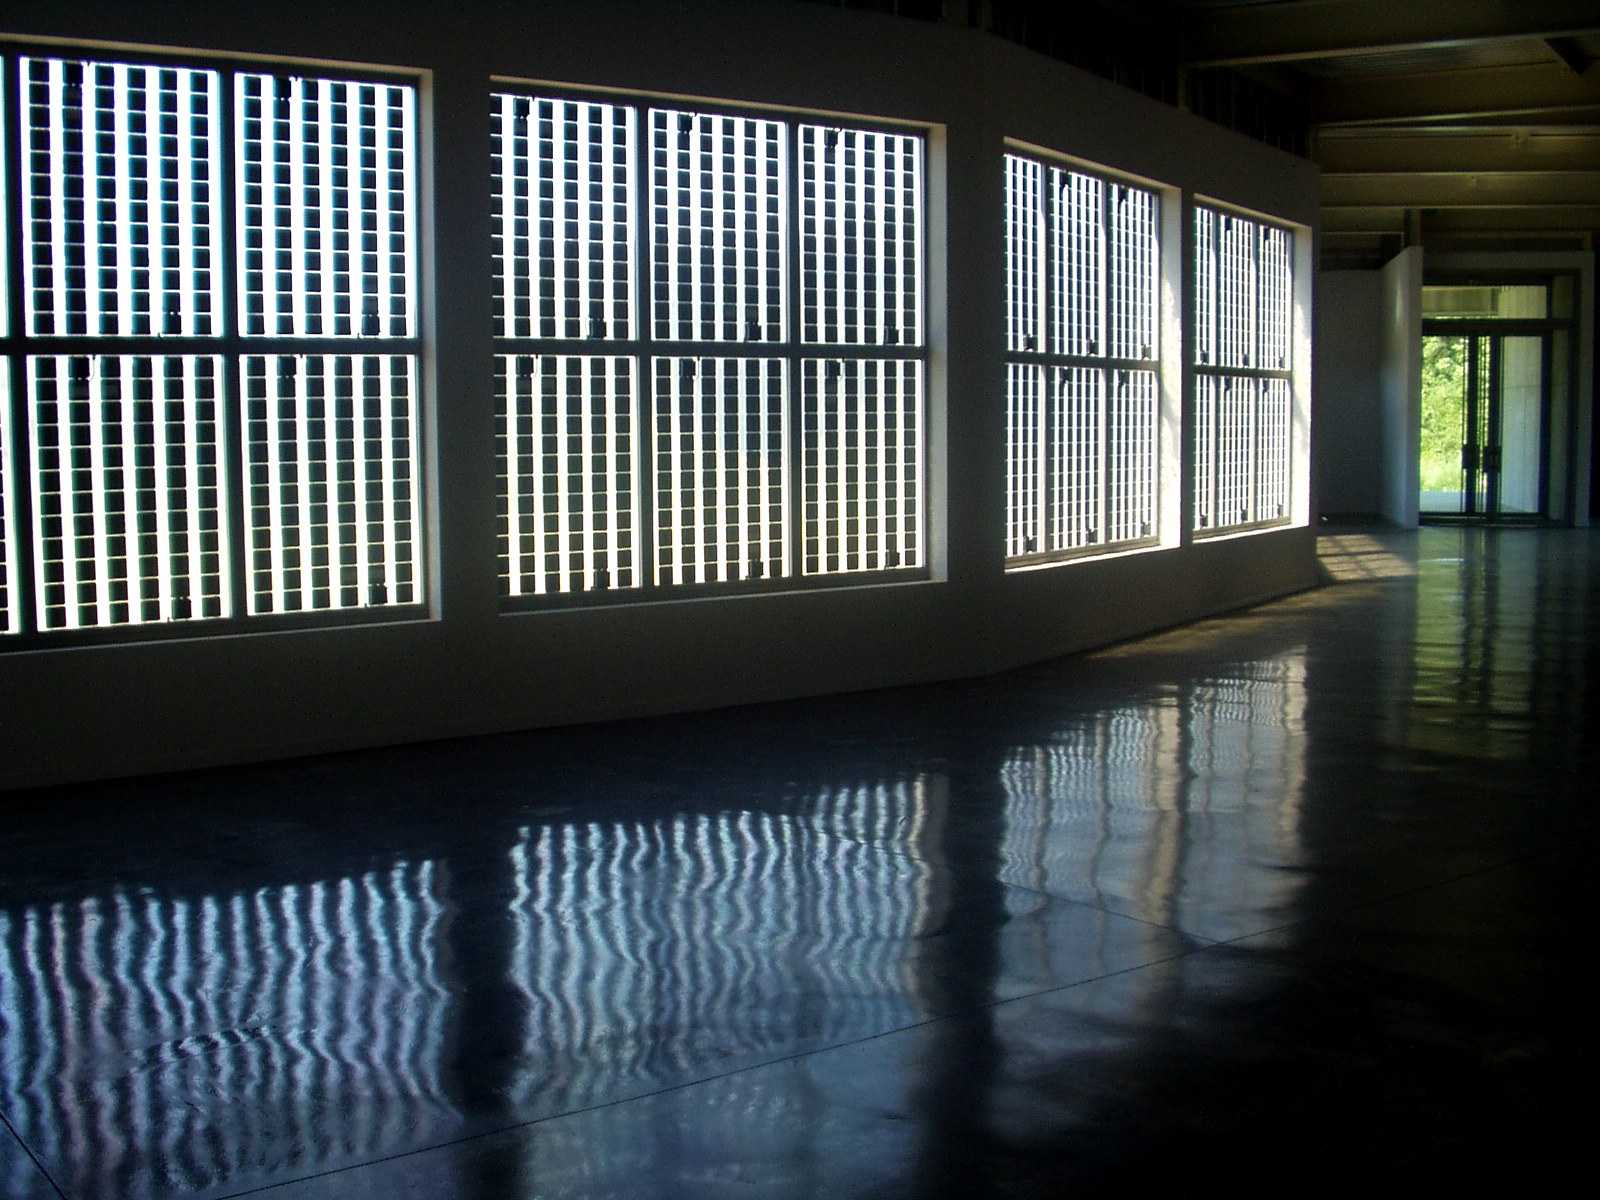
\includegraphics[width=.9\linewidth]{../figs/VistadesdeInterior.jpg}
\end{center}
\end{frame}
\end{document}